\pagenumbering{arabic}
%\setcounter{page}{1}
\chapter{Descriptive Statistics and an Introduction to R}
\index{Introduction}
\label{sec.matrix}
%start relabeling as 2.1 etc
\pagestyle{myheadings}  \markboth{\ref{sec.matrix}.
\titleref{sec.matrix}}{}
%\setcounter{equation}{0}

In this section, we will briefly introduce R, a useful tool for statistical computing and data visualisation, discuss quantitative data with its properties, basic statistical value calculation and box plot.\\

\section{Overview}

%\subsection{What is Statistics} \label{ssec.defm}\markright{\ref{ssec.defm} \titleref{ssec.defm}}

Intuitively, statistics can be considered the science of uncertainty. Formally,

\begin{definition}[Statistics]	\index{Statistics!Definition}
Statistics is the science of collecting, classifying, summarising, analysing and interpreting data.
\end{definition}

\subsection{Population, Sample, Parameter Statistics}

To begin with this course, here are more definitions that you should know.

\begin{definition}[Population]	\index{Population!Definition}
In statistics, a population is a set of similar items or events which is of interest for some question or experiment. It can be a group of existing objects for example the set of all students at UTM who have taken STA258, or a hypothetical group of objects conceived as a generalisation from experience for example the set of all possible combinations that selecting 2 numbers from 1 to 100.
\end{definition}

\begin{definition}[Sample]	\index{Sample}
A sample represents a subset of the cases and is often a small fraction of the population. For example, 100 students at UTM who have taken STA258.
\end{definition}

\begin{definition}[Parameter Statistics]	\index{Parameter Statistics}

\end{definition}

\subsection{Descriptive Statistics and Inferential Statistics}



\subsection{Qualitative Data and Quantitative Data}

\begin{definition}[Qualitative Data]	\index{Qualitative Data}
Qualitative data is non-numeric information, such as interview transcripts, diaries, notes and open-ended survey questions.
\end{definition}

\begin{definition}[Quantitative Data]	\index{Quantitative Data}
Quantitative data are data represented numerically, including anything that can be counted, measured, or given a numerical value. For example, STA258 final mark for 100 different students.
\end{definition}

\section{Descriptive statistics}

Descriptive statistics refers to the entire progress of summarising numerical and categorical data, then analysing those.\\ 

\noindent
\subsection{Sample Mean, Sample variance and Sample Standard Deviation}\\

\noindent
Sample mean is the average value of a sample of numbers taken from a population. Sample variance is a measure of dispersion in that sample which shows how far a set of numbers is spread out from sample mean. Sample standard deviation is a measure of the amount of variation of the values of a variable about its sample mean.

\begin{definition}
	Let $x_1, x_2, x_3, ..., x_n$ be a sample of data points. We define sample mean of the sample data points ($\bar{x}$) with n observations as the following: 
	$$ \bar{x} = \frac{1}{n} \sum_{i=1}^{n} x_i. $$
	Also, we define sample variance of the sample data points ($s^2$) as: \[ s^2 = \frac{1}{n-1} \sum_{i=1}^{n}(x_i - \bar{x})^2.\] Moreover, the standard deviation of the sample of data points ($s$) is: \[ s = \sqrt{s^2}, \quad \text{for } s > 0.\]
\end{definition}

Let's proceed with an example, to see how those values are calculated.

\begin{example}
Let: $x_1 = 1, x_2 = 3$ and $x_3 = 7$. Calculate the sample mean, sample variance and sample standard deviation for this collection of data points.\\

Solution (all results are kept in four digits):\\
\noindent
By Definition $1.2$, sample mean: \[ \bar{x} = \frac{1+3+7}{3} \approx 3.6667.\]
Then, we use sample mean to calculate sample variance: \[ s^2 = \frac{1}{3-1} \times [(1-3.6667)^2+(3-3.6667)^2+(7-3.6667)^2] \approx 9.3333.\]
Finally, we take the square root of sample variance to get sample deviation, and remember that $s > 0$: \[ s = \sqrt{s^2} \approx 3.0551.\]
\end{example}

\subsection{Median and Mode}\\

\noindent
Median indicates the information about the central value of a given collection of data points. Mode refers to a value which appears most frequently in a dataset.\\

\noindent
\textbf{Median:}
\begin{definition}
Let: $x_1, x_2, x_3, ... , x_n$ be a collection of data points which is arranged in ascending order from the smallest value to the largest value (or descending order from the largest value to the smallest value in that collection). The median of the given collection of data points is the middle value in that collection, which equally spreads the collection into two parts. Half of all the collection values are above the median value and the rest of the values in the collection is below the median value.
\begin{itemize}
 \item Case 1: when n is an odd number. (i.e. $1, 3, 11, 237,...$). Then, the median $M$ is defined as: \[ M = \frac{n+1}{2} \text{, where n represents the $n^{th}$ position}.\]
 \item Case 2: when n is an even number (i.e. $2, 6, 100, 500,...$). Then, the median $M$ is: the average value of $\frac{n}{2}$'s and $\frac{n+2}{2}$'s position, where n represents the $n^{th}$ position.
 \end{itemize}
\end{definition}
\begin{example}
Given two distinct collections of data points: $S_1$ = $\{2, 4, 6\}$ and $S_2$ = $\{1, 5, 16, 28\}$. Calculate the median of both two sets.\\
Solution: \\
For $S_1$, since $n = 3$ which is an odd number, so by $Definition \text{ } 1.3$, $M_{S_1} = 4$. For $S_2$, $n = 4$ in this case, so that we need to calculate the average of $\frac{n}{2}$ and $\frac{n+1}{2}$. Then, \[ M_{S_2} = \frac{5+16}{2} = 10.5.\]
\end{example}

\noindent
\textbf{Mode}
\begin{definition}
The mode of a dataset is a value which appears most frequently in it
\end{definition}

\begin{example}
Consider a dataset: $\{1, 2, 2, 3, 3, 3, 4, 4, 4, 4\}$. Find the mode of this dataset.\\
Solution:\\
Since '4' appears 4 time in the set, which is the most frequent. Thus, the mode of this given dataset is: 4.
\end{example}

\subsection{Percentile and Quartile}\\

\noindent
In statistics, percentiles and quartiles are tools used to describe the relative standing of data points within a dataset. They help us understand how individual values compare to the rest of the data.

\begin{definition}
Let: $x_1, x_2, ..., x_n$ be a collection of data points in either ascending order. Percentile is denoted as: $p^{th}$, which indicates $p \%$ of observations are below to a such value. Quartiles, which equally spread the collection of data into four parts. Each part contains $25\%$ of the entire collection. More specifically, we define quartiles as the following:
\begin{itemize}
 \item $Q_1$: the $25$ percentile (or $25^{th}$), which shows that $25\%$ of the data points are below the value $Q_1$.
 \item $Q_2$: the $50$ percentile (or $50^{th}$), which shows that $50\%$ of the data points are below the value $Q_2$.
 \item $Q_3$: the $75$ percentile (or $75^{th}$), which shows that $75\%$ of the data points are below the value $Q_3$.
 \item $Q_2$ is qual to median.
\end{itemize}
Moreover, we use $Q_3 - Q_1$ to calculate interquartile range (I.P.R), which shows the spread of the whole data set.
\end{definition}
 
 \begin{example}
Consider the data set $S = $ $\{4, 25, 30, 30, 30, 32, 32, 35, 50, 50, 50, 55, 60, 74, 110\}$. Calculate its median and $Q_1$ ($25^{th}$).\\
Solution:\\
Simply counting the number of data points, $n = 15$, such that $M_{S}$ = $\frac{15 + 1}{2}$ = $8$. Thus, the $8^{th}$ value in the set which is $35$.\\
Since we know the median of this collection of data points, we just need to find the median of the lower half of this data, which is exactly going to be $25$ percentile ($25^{th}$). In the lower half of the given collection (all values below the median), $n_{lower} = 7$. By $Definition \text{ } 1.3$, then median of the lower half ($25^{th}$) is going to be: \[ 25^{th} = \frac{7+1}{2} = 4, \text{ the $4^{th}$ position in the data set}.\] Thus, $Q_1$ ($25^{th}$) $= 30$. To find $Q_3$ ($75^{th}$), apply the same strategy will guide you to find the correct answer, and we leave this as an exercise to you.
\end{example}

\textbf{Five Number Summery}\\

\noindent
The five number summery are: minimum, $Q1$, $Q2$, $Q3$ and maximum.


\subsection{Skewness and Symmetry}\\

In probability theory and statistics, the word 'skewness' is a measure of the asymmetry of the probability distribution of a real-valued random variable about its mean. There are two types of skewness: left skewed (or negative skew) and right skewed (or positive skew).\\

\noindent
\textbf{Left Skewed (Negative Skew)}\\

\noindent
For a probability distribution of a real-valued random variable about its mean to be left skewed or negative skewed, we observe the tail of its graph, where the tail locates on the left. (See figure $1.1$ below)

\begin{figure}[H]
 \centering
 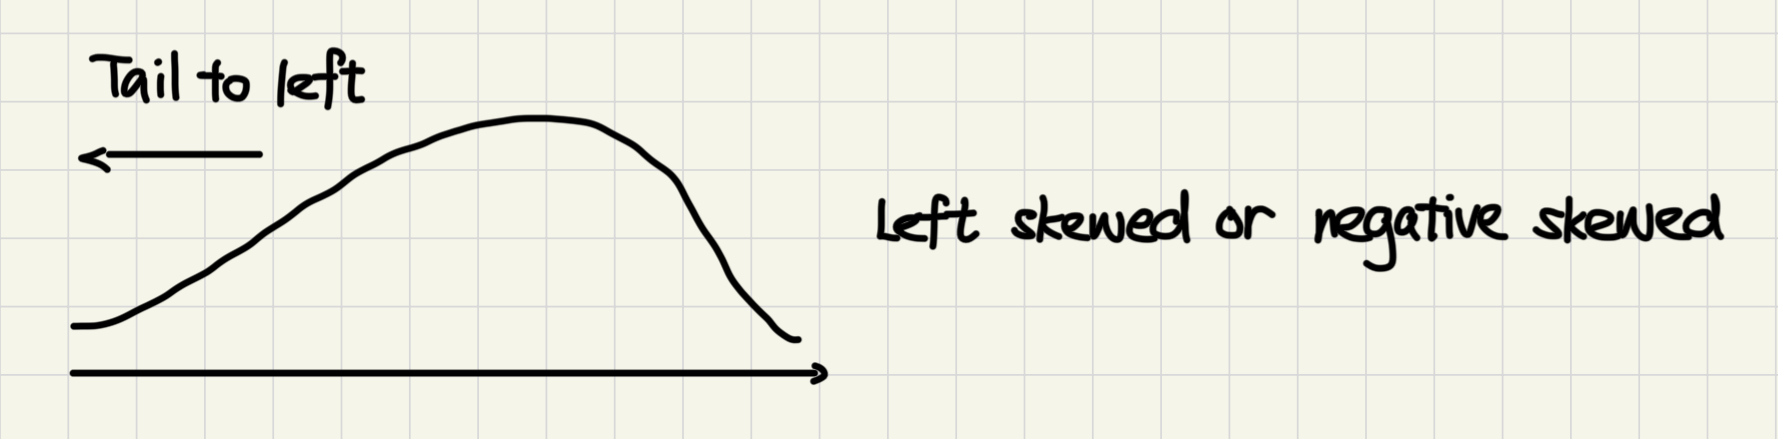
\includegraphics[scale=0.25]{Section1/img/LeftSkewed.jpg}
 \caption{Visualization of a left skewed distribution}
\end{figure}

\noindent
\textbf{Right Skewed (Positive Skew)}\\

\noindent
Similarly, if a probability distribution of a real-valued random variable about its mean has graph where its tail locates on the right, then we say that distribution is right skewed or positive skewed. (See figure 1.2 below)

\begin{figure}[H]
 \centering
 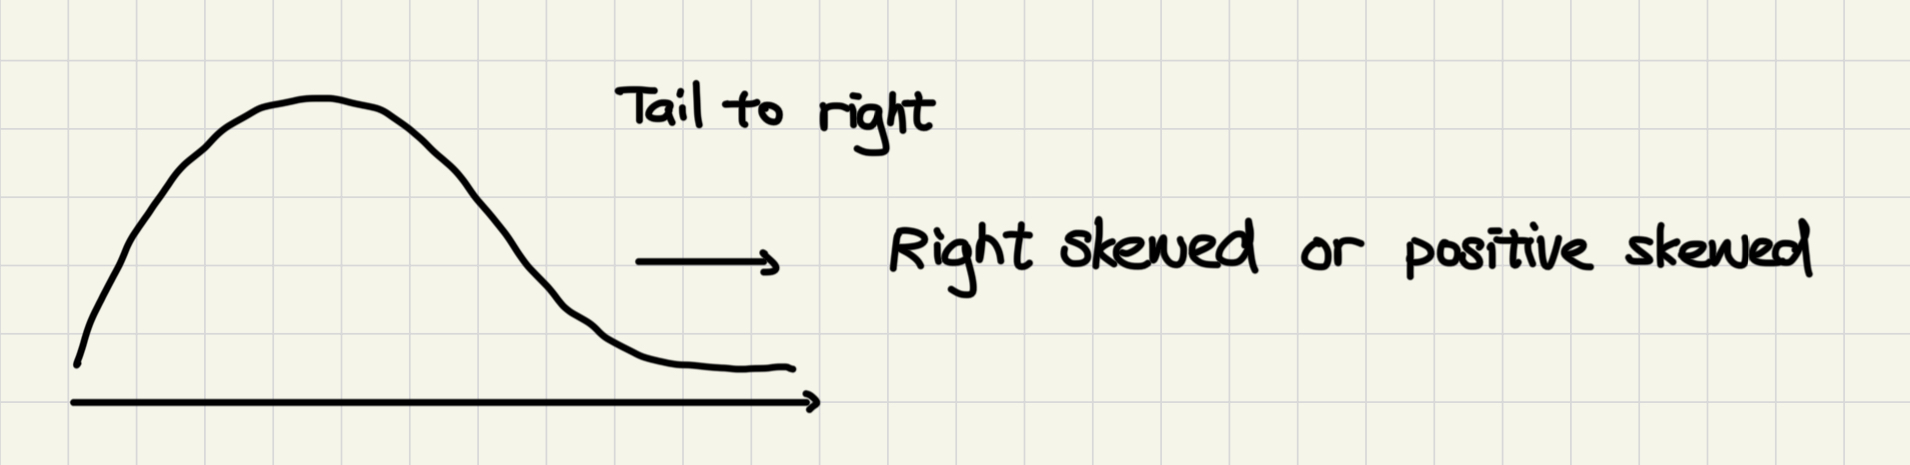
\includegraphics[scale=0.25]{Section1/img/RightSkewed.jpg}
 \caption{Visualization of a right skewed distribution}
\end{figure}

\noindent
Two classic example of right skewed probability distribution is $\chi^{2}$-distribution and F-distribution.\\

\noindent
\textbf{Symmetry}\\

\noindent
In statistics, a symmetric probability distribution is reflected around a vertical line at a certain value. That means the probability on the left side of that line at a certain point is equal to the probability on the right. (See figure 1.3 below)

\begin{figure}[H]
 \centering
 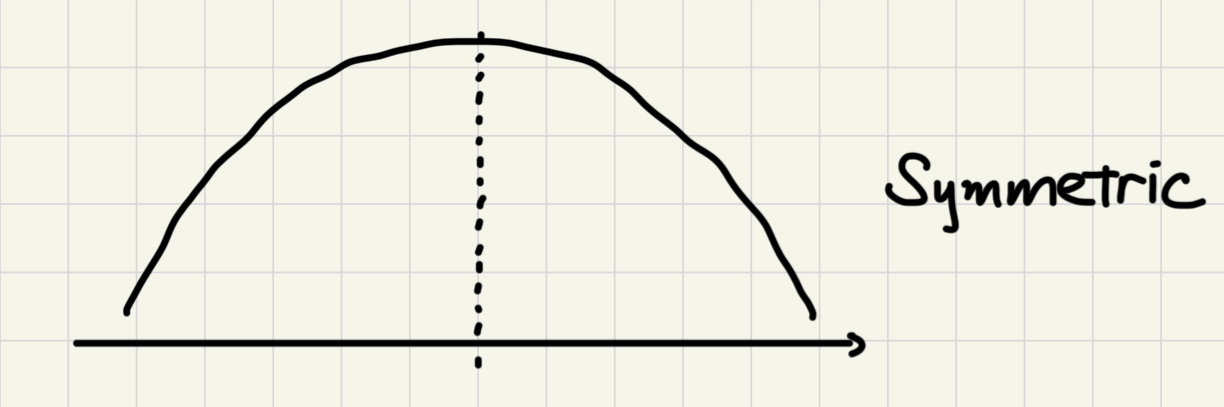
\includegraphics[scale=0.25]{Section1/img/Symmetric.jpg}
 \caption{Visualization of a symmetric distribution}
\end{figure}

\noindent
Some common examples of symmetric probability distribution in real world are: normal distribution and student's t-distribution.\\

\noindent
\textbf{The Empirical Rule}
\begin{definition}[The Empirical Rule or $68-95-99.7$ Rule]
  For any symmetric (bell-shaped) curve, let $\mu$ be its mean and $\sigma$ be its standard deviation, the following probability set function is true:
   \begin{itemize}
    \item  $1.$: $Pr(\mu - \sigma < X < \mu + \sigma) = 68.27\%;$
    \item  $2.$: $Pr(\mu - 2\sigma < X < \mu + 2\sigma) = 95.45\%;$
    \item  $3.$: $Pr(\mu - 3\sigma < X < \mu + 3\sigma) = 99.73\%.$
   \end{itemize}
  \end{definition}

\section{Graphical Techniques}\\

\noindent
In this section, we are going to introduce some common statistical graphs. Then, we will obtain information and do interpretation from the graphs.

\subsection{Histograms}\\

\noindent
A histogram is constructed by placing the variables of interest on the horizontal axis and the frequency, relative frequency, or percent frequency on the vertical axis, which is a type of quantitative or numerical data for statistical analysis. For example: STA258 final mark from 100 different students at UTM. The following figure is an example of histogram: 

\begin{figure}[H]
 \centering
 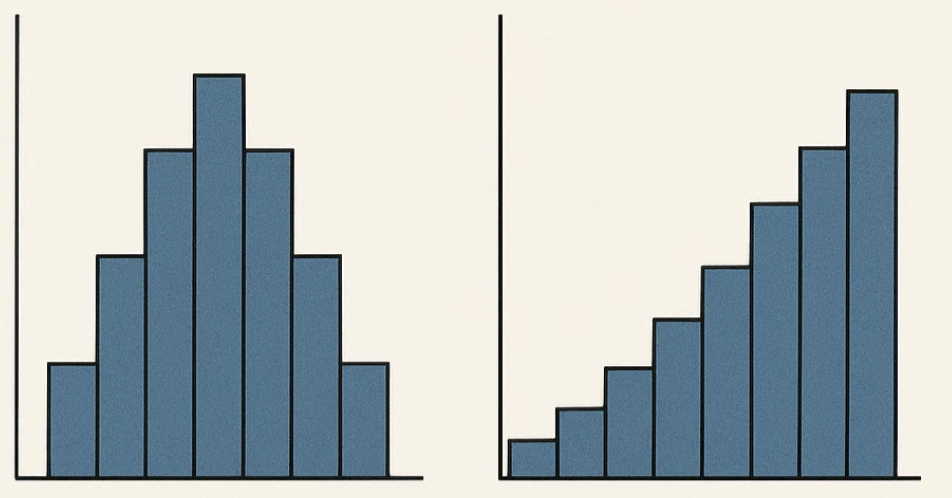
\includegraphics[scale=0.15]{Section1/img/Histogram.jpg}
 \caption{Visualization of a histogram: its horizontal axis lists the bins of a data, its vertical axis represents the frequency of the occurance}
\end{figure}

\noindent
\textbf{Advantages and Disadvantages of Histograms}

\begin{itemize}
 \item Advantages:\\
 $1.$ Histograms are easily to used for visualise data (relatively). It allows us to get the idea of the "shape" of distribution (i.e. skewness which will be discussed late in this section).\\
 $2.$ It is also flexible that people are able to modify bin widths.
 \item Disadvantages:\\
 $1.$ It is not suitable for small data sets.\\
 $2.$ The values from histograms close to breaking points are likely similar, in fact they need to be classified into different bins (i.e. Student A and B scores 79 and 80 respectively in STA258, we consider a breaking point between 79 and 80. The two students have similar score, but student A is $B^+$ and student B is $A^-$ in GPA from).
\end{itemize}

\noindent
\textbf{Histograms Relate to Skewness and Symmetry}\\

\noindent
We can determine skewness and symmetry by observing and drawing a curve above columns on histograms. We use this method to approximate the shape of probability distribution baed on histograms. As the following figures show:

\begin{figure}[H]
 \centering
 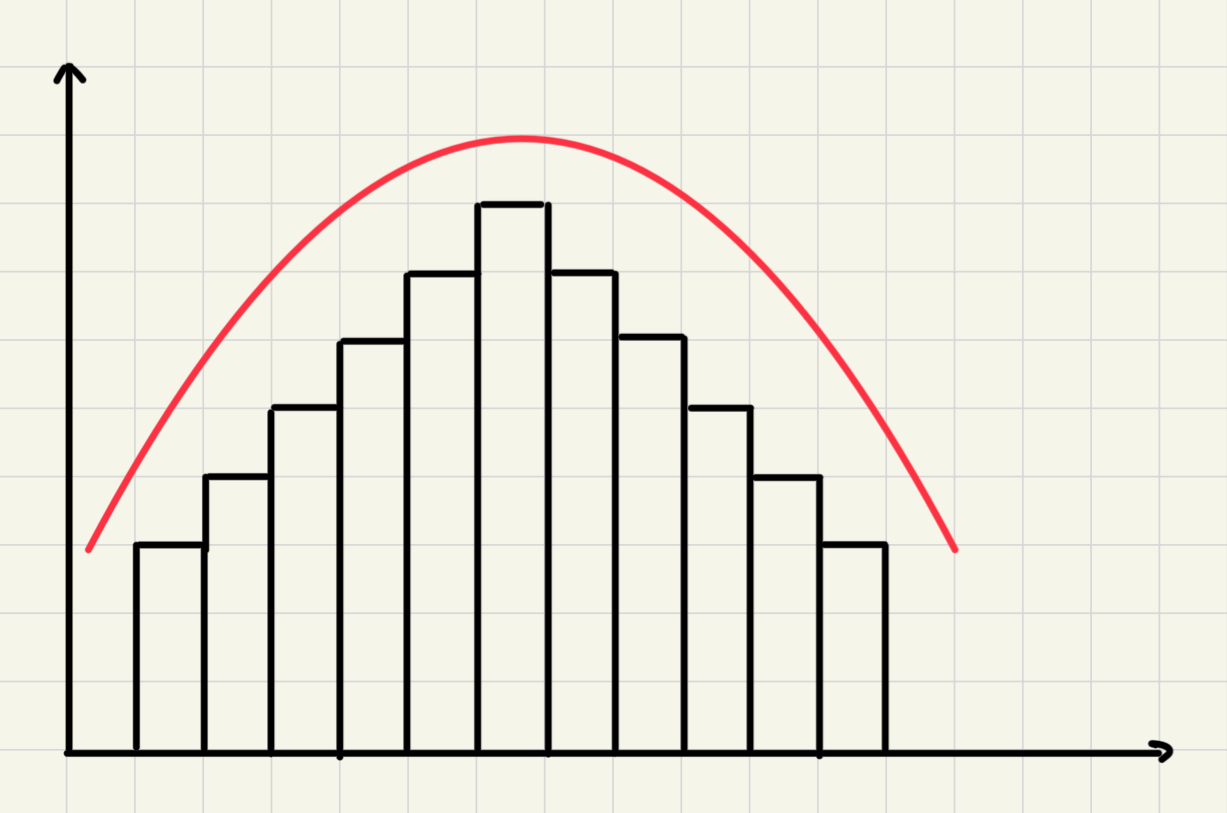
\includegraphics[scale=0.15]{Section1/img/HisSymm.jpg}
 \caption{Visualisation of a histogram with approximate symmetric probability distribution}
\end{figure}

\begin{figure}[H]
 \centering
 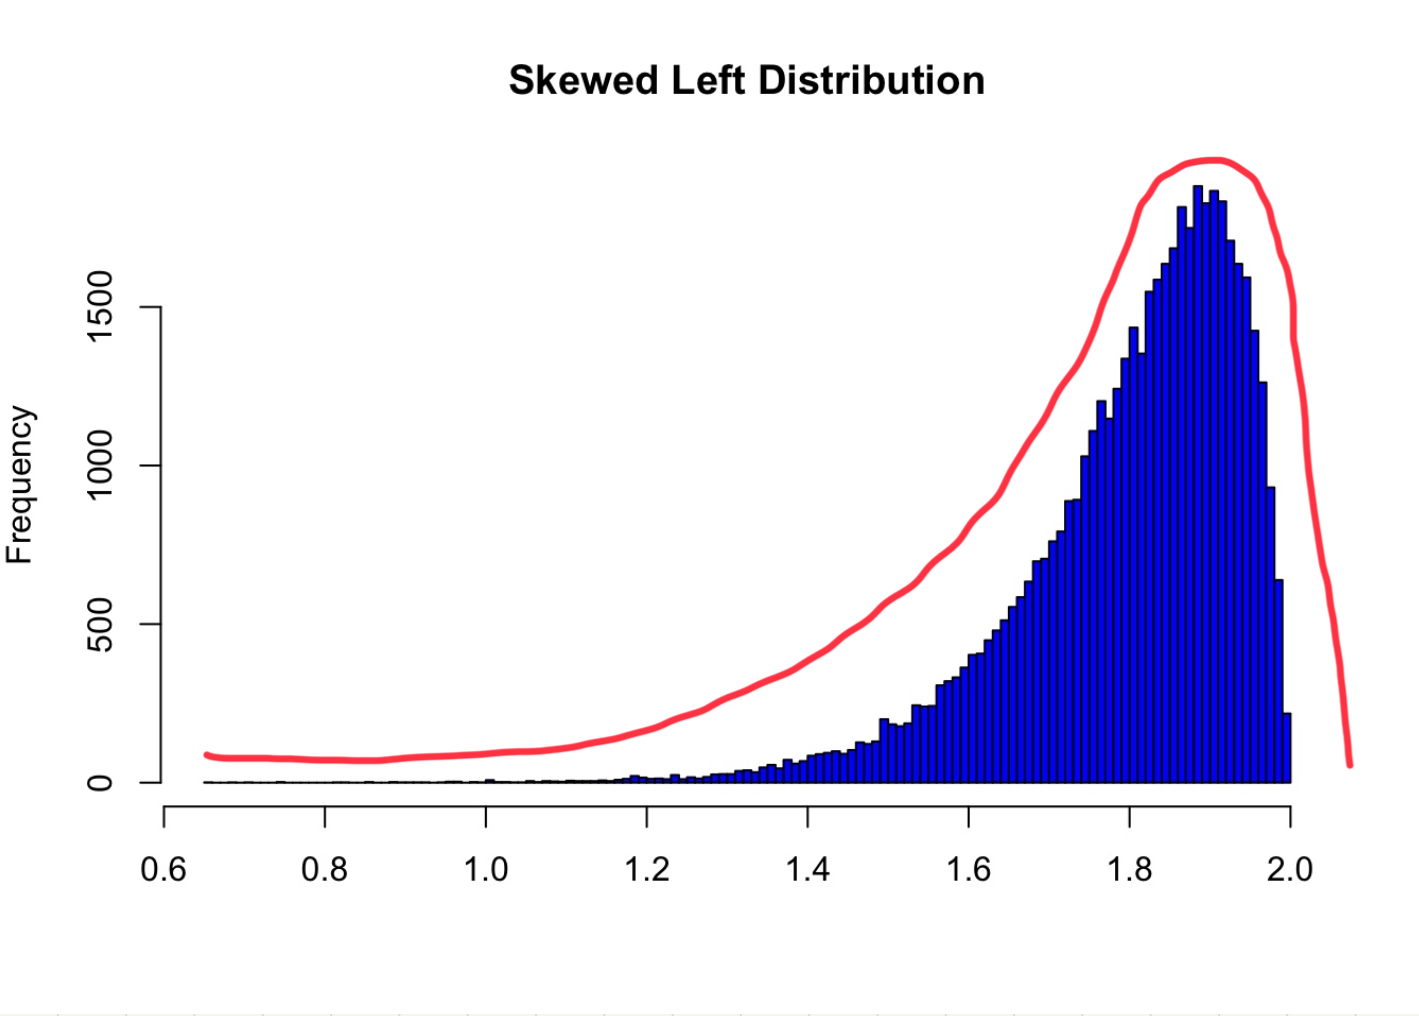
\includegraphics[scale=0.15]{Section1/img/HisL.jpg}
 \caption{Visualisation of a histogram with approximate left skew probability distribution}
\end{figure}

\begin{figure}[H]
 \centering
 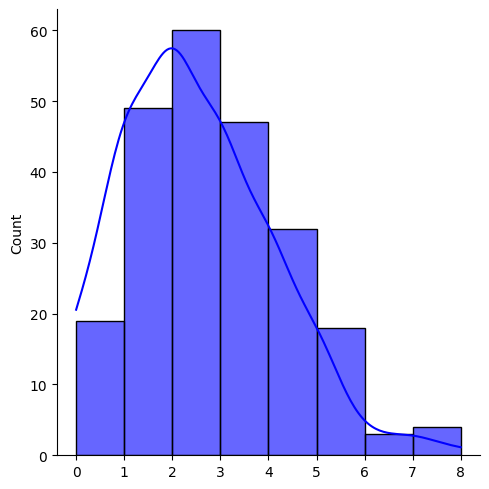
\includegraphics[scale=0.35]{Section1/img/HisR.jpg}
 \caption{Visualisation of a histogram with approximate right skew probability distribution}
\end{figure}

\subsection{Box Plot}\\

\noindent
In descriptive statistics, we use box plot to demonstrating graphically the locality, spread and skewness groups of numerical data through their quartiles. Let's use a figure to demonstrate a box plot. 

\begin{figure}[H]
 \centering
 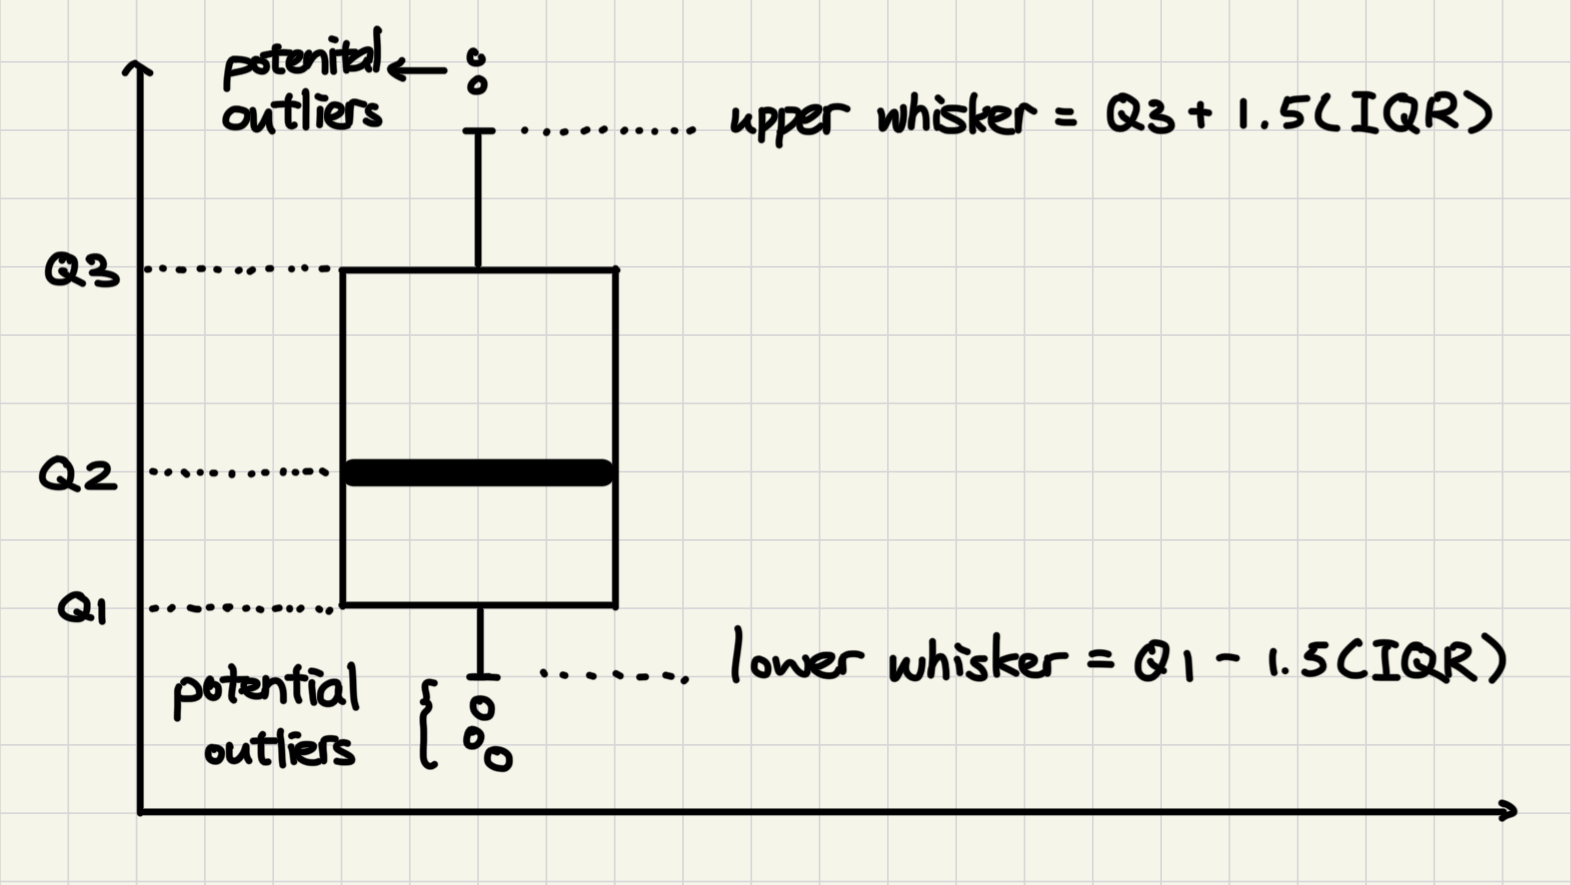
\includegraphics[scale=0.30]{Section1/img/Boxplot.jpg}
 \caption{Visualisation of a box plot}
\end{figure}

In this course, we should be able to obtain some key values to help us to continue our statistical analysis. These values are: minimum, $Q1$, $Q2$ (median), $Q3$, maximum and outliers.\\

\noindent
\textbf{Box Plot and Skewness of Probability Distribution}\\

\noindent
We can obtain skewness from box plot as well. From box plot instead of drawing a curve, we observe how median ($Q2$) separates the 'box' in box plot. In words, if median is greater than mean in a box plot, then it has a negative skewed probability distribution. Otherwise, if median is less than mean in a box plot, then it has a positive skewed probability distribution. However, when median is equal to mean in a box plot, then it has a symmetric probability distribution. (See figure below)

\begin{figure}[H]
 \centering
 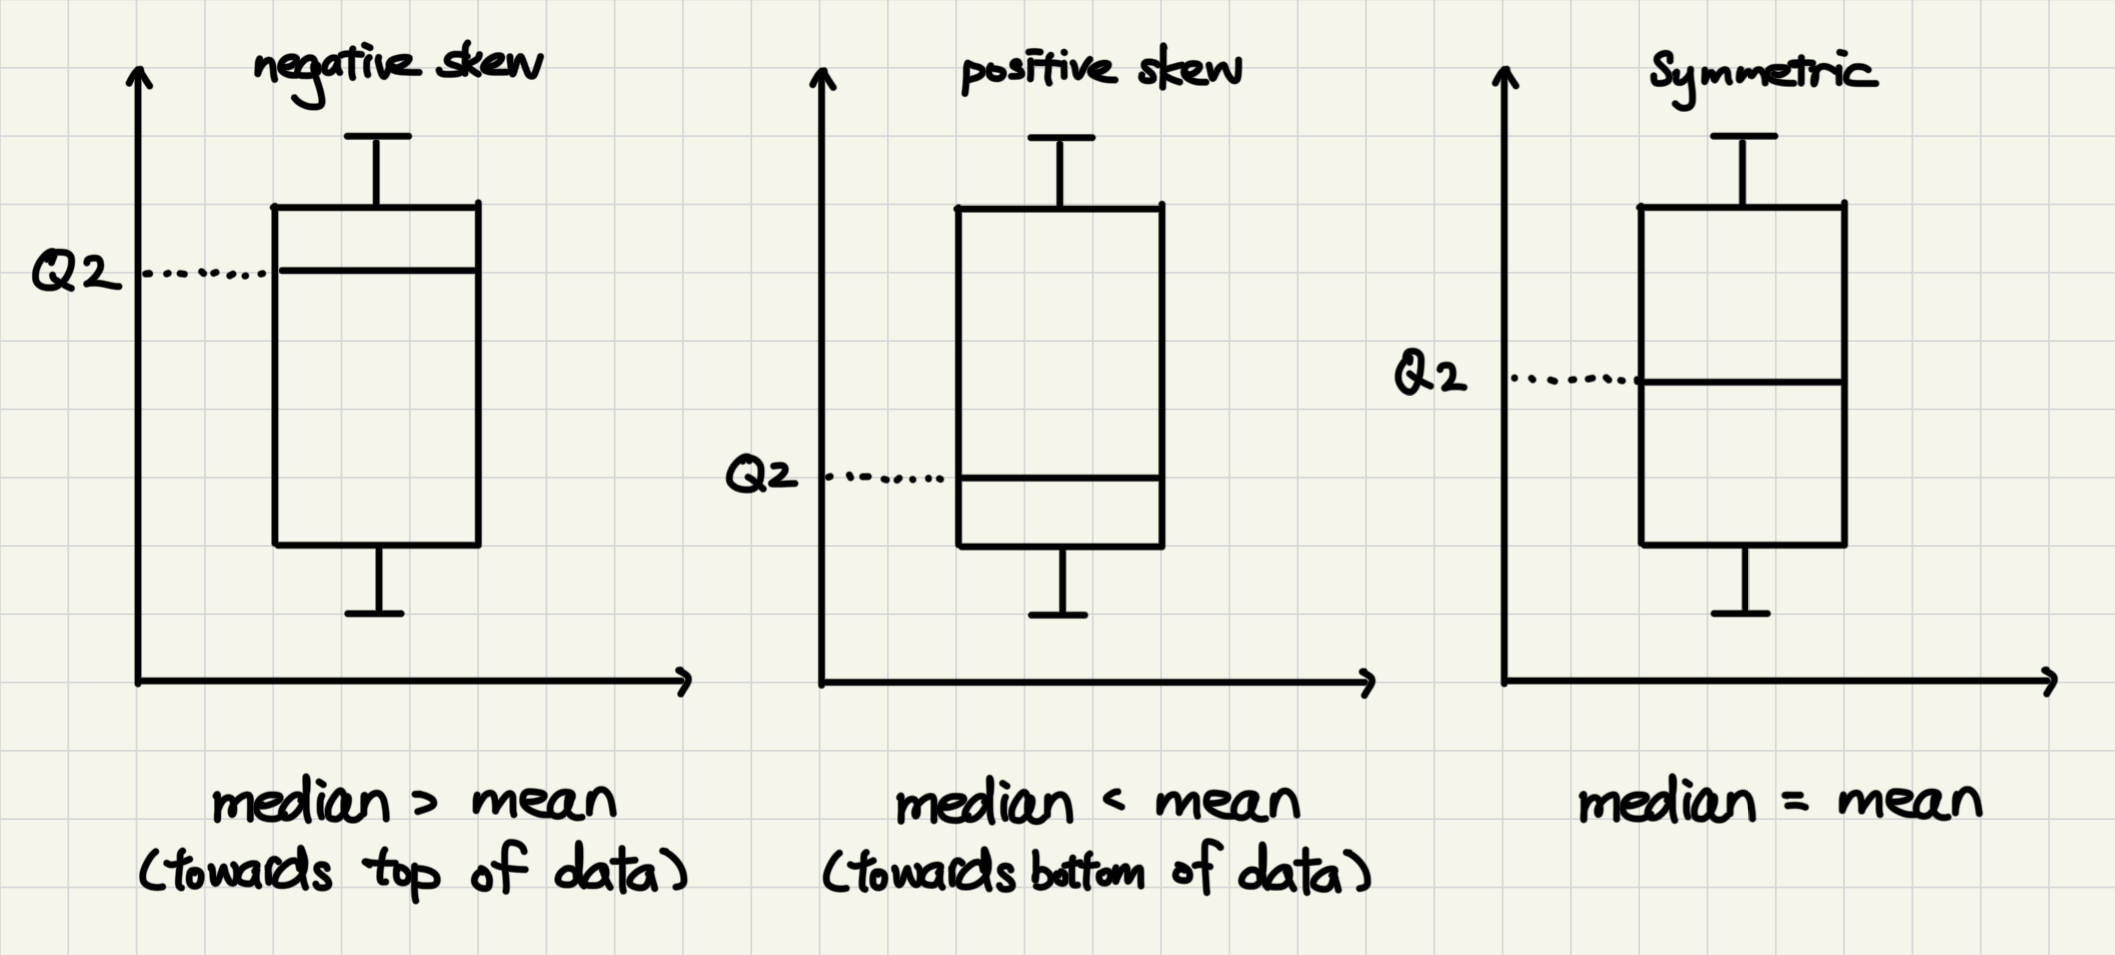
\includegraphics[scale=0.20]{Section1/img/BoxSk.jpg}
 \caption{Visualisation of how to obtain skewness and symmetry from a box plot}
\end{figure}

\section{Introduction to R}\\

\noindent
R is used for data manipulation, statistics, and graphics. It is made of: operations ($+$,$ -$, $<$) which is for calculations on vectors, arrays and matrices; a huge collection of functions; facilities for making unlimited types quality graphs; user contributed packages (sets of related functions); the ability to interface with procedures written in C, C+, or FORTRAN and to write additional primitives. R is also an open-source computing package which has seen a huge growth in popularity in the last few years (Please use this website: https://cran.r-project.org, to download R).\\

\noindent
\textbf{What is R-studio?}\\

\noindent
RStudio is a relatively new editor specially targeted at R. RStudio is cross-platform, free and open-source software (Please use: https://www.rstudio.com, to download Rstudio).






